\section{Comparative Analysis \& Advanced Topics}

\begin{frame}{Equation-Based vs.\ Agent-Based Models}
  \small
  \begin{center}
  \begin{tabular}{p{3.2cm}p{4cm}p{4cm}}
    \toprule
    \textbf{Aspect} & \textbf{Equation-Based} & \textbf{Agent-Based} \\
    \midrule
    \textbf{Unit of analysis} & Populations (fractions) & Individual agents \\
    \textbf{State variables} & Continuous ($S$, $I$, $R$) & Discrete per agent \\
    \textbf{Stochasticity} & Deterministic (by default) & Inherently stochastic \\
    \textbf{Spatial structure} & Well-mixed (homogeneous) & Explicit space \\
    \textbf{Heterogeneity} & Hard to include & Natural \\
    \textbf{Computation} & Very fast (ODEs) & Slower (per-agent loops) \\
    \textbf{Analytical results} & Often possible ($R_0$, stability) & Rarely possible \\
    \bottomrule
  \end{tabular}
  \end{center}
  \vfill
  \begin{block}{When to use which?}
    \begin{itemize}
      \item Use \textbf{ODE models} for quick qualitative insight and analytical results.
      \item Use \textbf{ABMs} when individual variation, space, or networks matter.
    \end{itemize}
  \end{block}
\end{frame}

\begin{frame}{Comparing SIR Curves: ODE vs.\ ABM}
  \begin{center}
    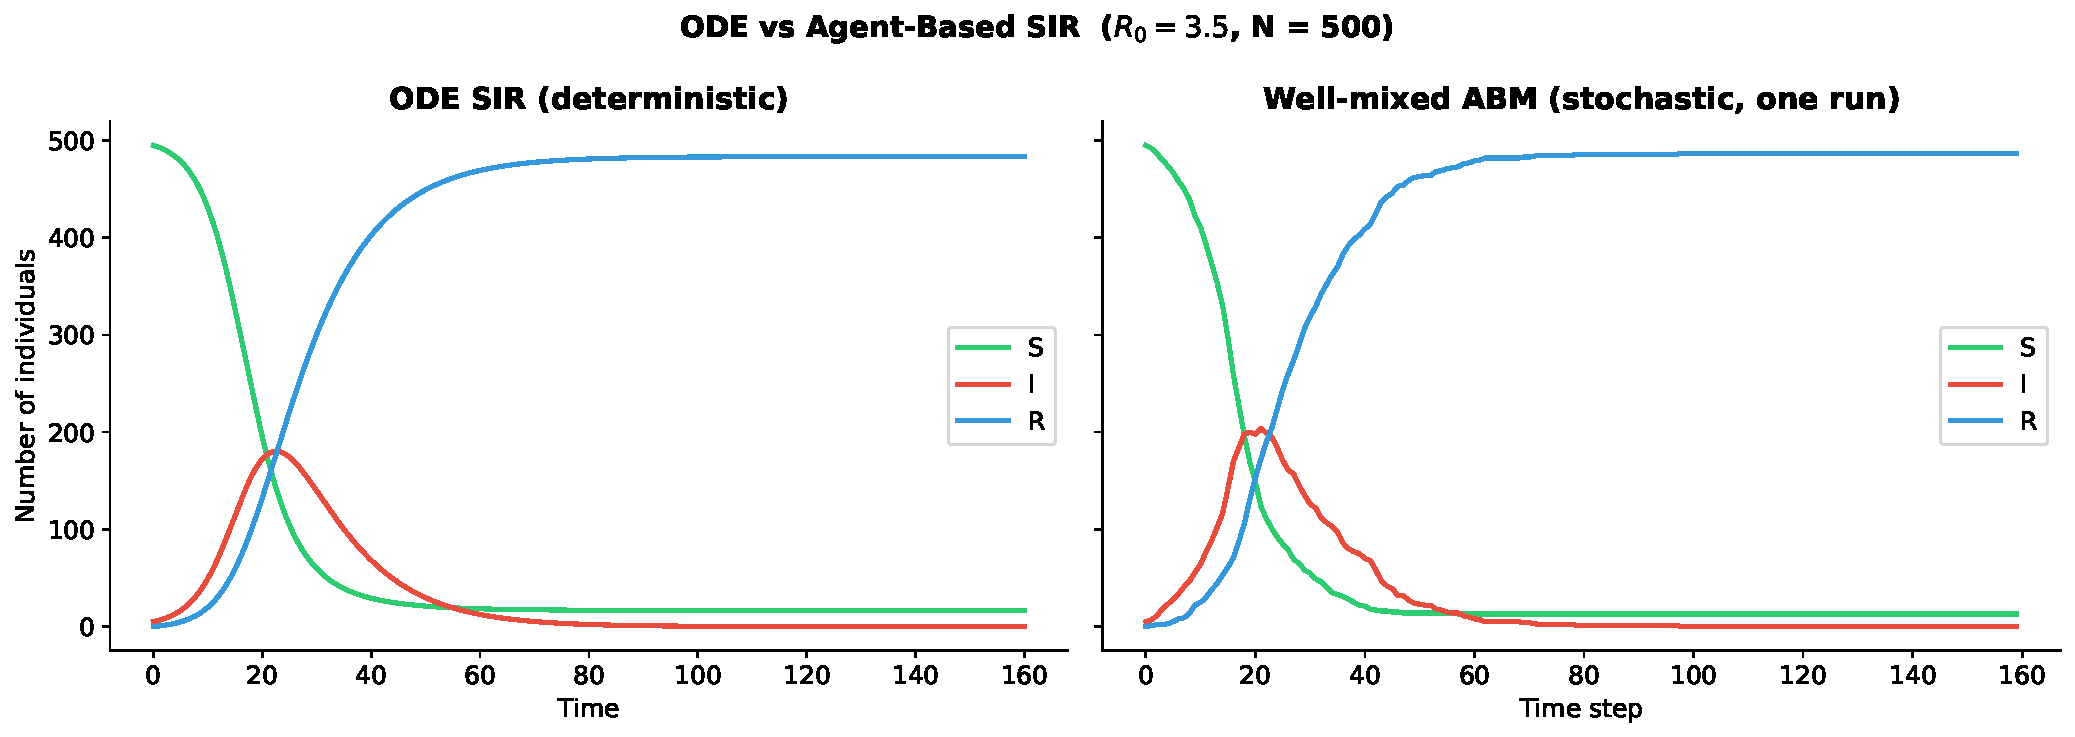
\includegraphics[width=0.9\textwidth]{images/ode_vs_abm.pdf}
  \end{center}
  \small
  The ODE model (smooth curves) represents the mean-field limit.  
  The ABM (noisy lines) shows the stochastic reality for finite populations.
\end{frame}

\begin{frame}{Stochastic Variability in the ABM}
  \begin{center}
    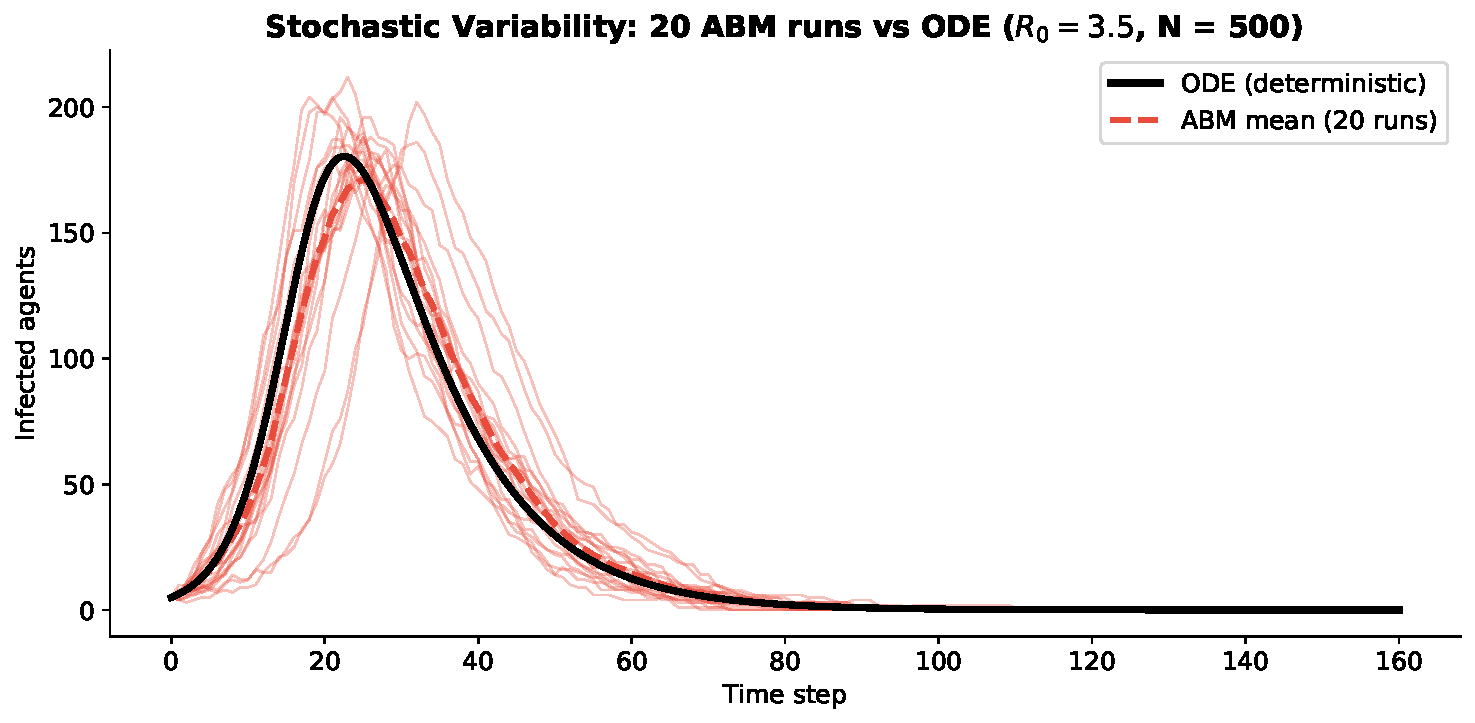
\includegraphics[width=0.85\textwidth]{images/abm_variability.pdf}
  \end{center}
  \small
  Multiple ABM runs with identical parameters but different random seeds produce different outbreak sizes. The ODE solution is the deterministic ``average'' trajectory.
\end{frame}

\begin{frame}{Effect of Population Size}
  \begin{itemize}
    \item With \textbf{small populations}, randomness dominates --- outbreaks may fizzle out even when $R_0 > 1$.
    \item With \textbf{large populations}, the ABM converges toward the ODE solution (\textbf{law of large numbers}).
    \pause
    \item The probability that an epidemic takes off in a stochastic model is approximately:
    \[
      P_{\text{outbreak}} \approx 1 - \frac{1}{R_0}
    \]
    for a single initial infected individual.
  \end{itemize}
  \vfill
  \begin{center}
    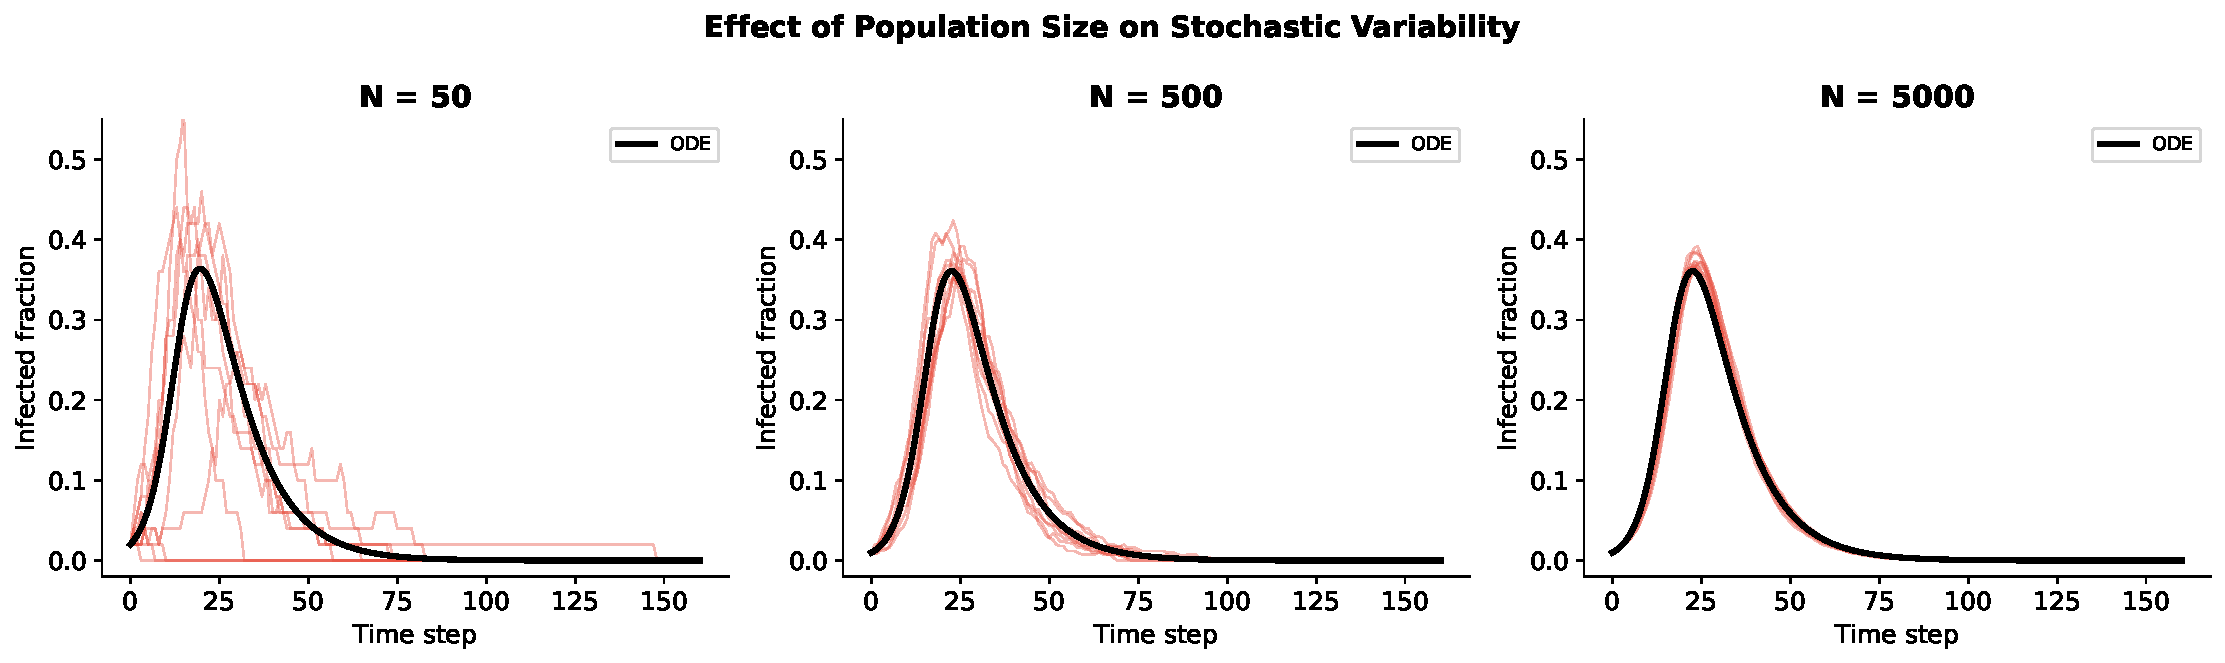
\includegraphics[width=0.75\textwidth]{images/population_size_effect.pdf}
  \end{center}
\end{frame}

\begin{frame}{Network Structure and Disease Spread}
  \begin{itemize}
    \item In the ODE model, we assume a \textbf{well-mixed} population (everyone contacts everyone).
    \item In reality, contacts are structured: families, workplaces, schools, transport.
    \item Network topology strongly affects epidemic dynamics:
  \end{itemize}
  \vfill
  \begin{center}
    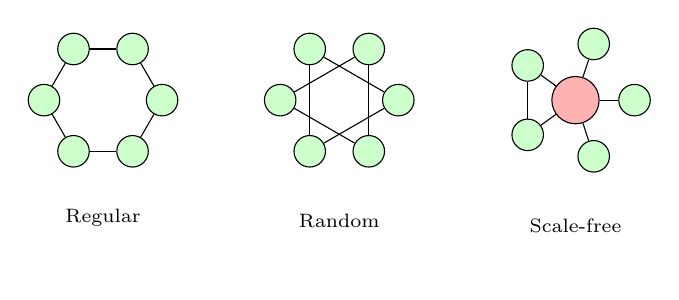
\begin{tikzpicture}[scale=0.5, every node/.style={draw, circle, fill=green!20, minimum size=0.4cm, inner sep=0pt}]
      % Regular lattice
      \begin{scope}[shift={(-6,0)}]
        \foreach \i in {1,...,6} {
          \pgfmathsetmacro{\ang}{60*\i}
          \node (a\i) at (\ang:1.5) {};
        }
        \foreach \i in {1,...,5} {
          \pgfmathtruncatemacro{\j}{\i+1}
          \draw (a\i) -- (a\j);
        }
        \draw (a6) -- (a1);
        \node[draw=none, fill=none, below, font=\scriptsize] at (0,-2) {Regular};
      \end{scope}
      % Random
      \begin{scope}[shift={(0,0)}]
        \foreach \i in {1,...,6} {
          \pgfmathsetmacro{\ang}{60*\i}
          \node (b\i) at (\ang:1.5) {};
        }
        \draw (b1) -- (b3); \draw (b1) -- (b5); \draw (b2) -- (b4);
        \draw (b2) -- (b6); \draw (b3) -- (b5); \draw (b4) -- (b6);
        \node[draw=none, fill=none, below, font=\scriptsize] at (0,-2) {Random};
      \end{scope}
      % Scale-free
      \begin{scope}[shift={(6,0)}]
        \node[fill=red!30, minimum size=0.6cm] (c1) at (0,0) {};
        \foreach \i in {2,...,6} {
          \pgfmathsetmacro{\ang}{72*\i}
          \node (c\i) at (\ang:1.5) {};
          \draw (c\i) -- (c1);
        }
        \draw (c2) -- (c3);
        \node[draw=none, fill=none, below, font=\scriptsize] at (0,-2) {Scale-free};
      \end{scope}
    \end{tikzpicture}
  \end{center}
  \small
  Scale-free networks (hubs) make epidemics spread faster and harder to contain.
\end{frame}

\begin{frame}{Vaccination Strategies}
  \begin{columns}
    \column{0.5\textwidth}
    \begin{itemize}
      \item \textbf{Random vaccination}: vaccinate a fraction $p$ of the population at random.
      \item Epidemic is prevented if $p > p_{\text{herd}} = 1 - 1/R_0$.
      \pause
      \item \textbf{Targeted vaccination}: vaccinate high-degree nodes (hubs) or high-contact individuals.
      \item Much more efficient on structured networks.
    \end{itemize}
    \column{0.5\textwidth}
    \begin{center}
      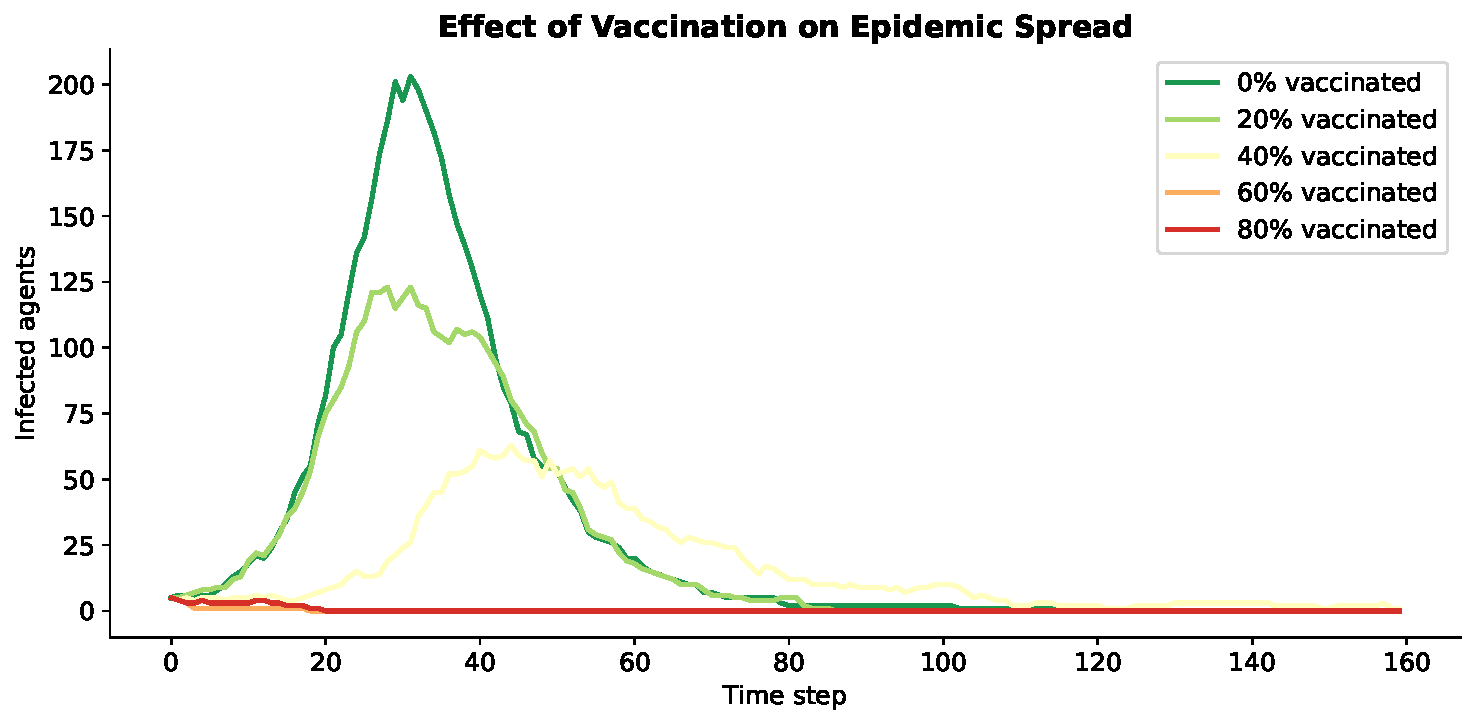
\includegraphics[width=\textwidth]{images/vaccination_effect.pdf}
    \end{center}
  \end{columns}
\end{frame}

\begin{frame}{The SEIR Model in Practice: COVID-19}
  \begin{center}
    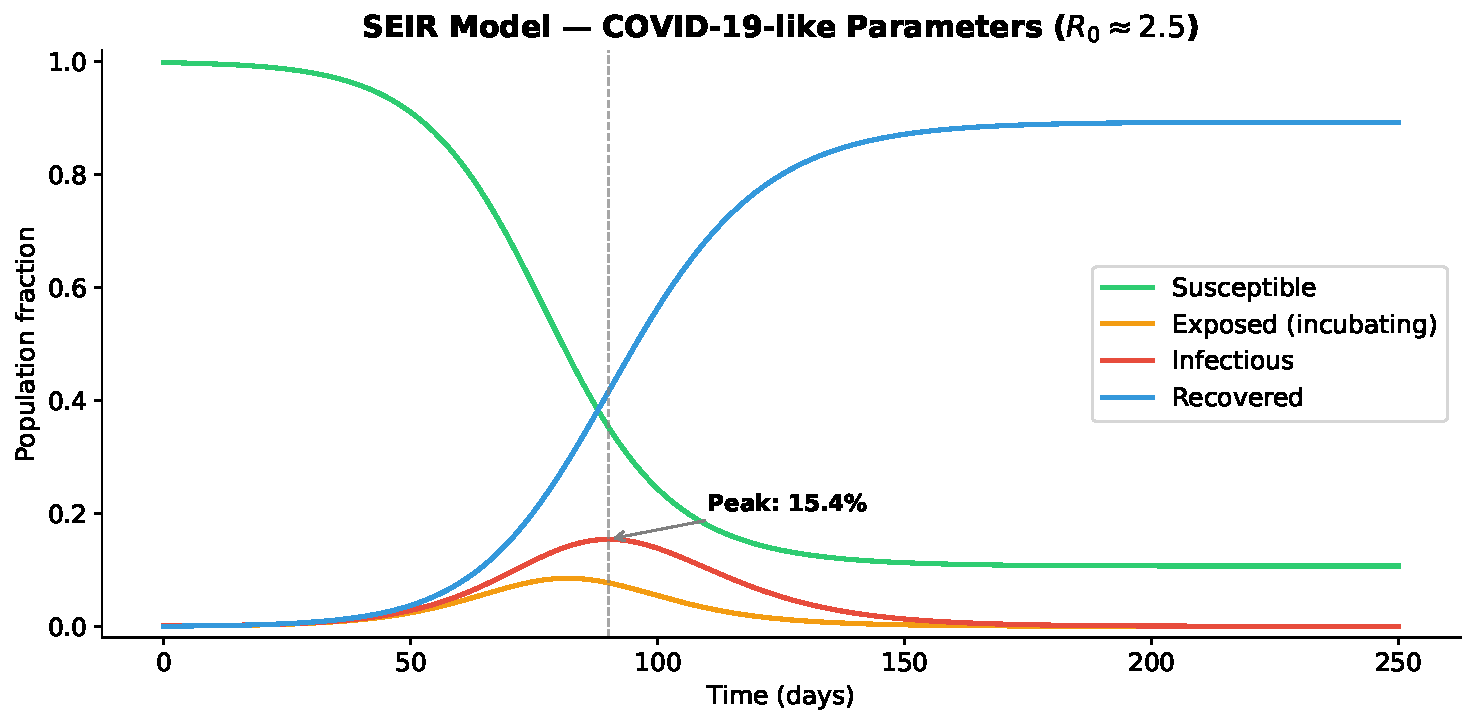
\includegraphics[width=0.85\textwidth]{images/seir_covid_example.pdf}
  \end{center}
  \small
  SEIR model fitted to early COVID-19 data. The exposed compartment captures the incubation period ($\approx 5$ days) before individuals become infectious.
\end{frame}

\begin{frame}{Summary of Epidemic Models}
  \begin{center}
  \footnotesize
  \begin{tabular}{lcccl}
    \toprule
    \textbf{Model} & \textbf{Compartments} & \textbf{Recovery?} & \textbf{Immunity?} & \textbf{Example disease} \\
    \midrule
    SI & 2 & No & No & Cytomegalovirus \\
    SIS & 2 & Yes & No & Common cold, gonorrhea \\
    SIR & 3 & Yes & Yes & Influenza, measles \\
    SEIR & 4 & Yes & Yes & COVID-19, Ebola \\
    \bottomrule
  \end{tabular}
  \end{center}
  \vfill
  \begin{itemize}
    \item All models share the same core idea: \textbf{compartments} connected by \textbf{transition rates}.
    \item The choice of model depends on the disease biology and the questions being asked.
    \item $R_0$ is the single most important parameter across all models.
  \end{itemize}
\end{frame}

\begin{frame}{Exercise: Compare Models}
  \begin{enumerate}
    \item Simulate the SIR model with $R_0 = 2.5$ using the equation-based approach. Record the peak infected fraction and the final size.
    \item Simulate the same scenario using the agent-based model with 500 agents. Run 10 different seeds.
    \item Compare the mean ABM outcome with the ODE result. How close are they?
    \item Reduce the population to 50 agents. How does variability change?
    \item Advanced: implement a simple vaccination strategy in the ABM and find the minimum vaccination coverage that prevents an outbreak.
  \end{enumerate}
\end{frame}
